\documentclass{standalone}
\usepackage{graphicx}	
\usepackage{amssymb, amsmath}
\usepackage{color}

\usepackage{tikz}
\usetikzlibrary{intersections, backgrounds}
\usepackage{pgfmath}

\definecolor{light}{RGB}{220, 188, 188}
\definecolor{mid}{RGB}{185, 124, 124}
\definecolor{dark}{RGB}{143, 39, 39}
\definecolor{highlight}{RGB}{180, 31, 180}
\definecolor{gray10}{gray}{0.1}
\definecolor{gray20}{gray}{0.2}
\definecolor{gray30}{gray}{0.3}
\definecolor{gray40}{gray}{0.4}
\definecolor{gray60}{gray}{0.6}
\definecolor{gray70}{gray}{0.7}
\definecolor{gray80}{gray}{0.8}
\definecolor{gray90}{gray}{0.9}
\definecolor{gray95}{gray}{0.95}

\begin{document}

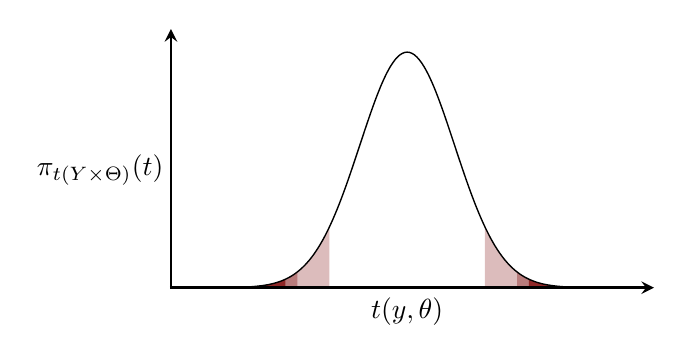
\begin{tikzpicture}[scale=0.3, thick,
declare function={ g(\x) = exp(-0.5 * (\x - 0) * (\x - 0) / (2 * 2)) / (2.506628274631001 * 2);}
]
  
  \begin{scope}
    \clip (-10, 0) rectangle (-3.289707, 10);
    \fill[color=light, domain=-10:10, smooth, samples=100, variable=\x] 
      plot ({\x}, {50 * g(\x)});
  \end{scope}
  
  \begin{scope}
    \clip (-10, 0) rectangle (-4.652696, 10);
    \fill[color=mid, domain=-10:10, smooth, samples=100, variable=\x] 
      plot ({\x}, {50 * g(\x)});
  \end{scope}
  
  \begin{scope}
    \clip (-10, 0) rectangle (-5.151659, 10);
    \fill[color=dark, domain=-10:10, smooth, samples=100, variable=\x] 
      plot ({\x}, {50 * g(\x)});
  \end{scope}

  \begin{scope}
    \clip (3.289707, 0) rectangle (10, 10);
    \fill[color=light, domain=-10:10, smooth, samples=100, variable=\x] 
      plot ({\x}, {50 * g(\x)});
  \end{scope}
  
  \begin{scope}
    \clip (4.652696, 0) rectangle (10, 10);
    \fill[color=mid, domain=-10:10, smooth, samples=100, variable=\x] 
      plot ({\x}, {50 * g(\x)});
  \end{scope}
  
  \begin{scope}
    \clip (5.151659, 0) rectangle (10, 10);
    \fill[color=dark, domain=-10:10, smooth, samples=100, variable=\x] 
      plot ({\x}, {50 * g(\x)});
  \end{scope}
  
  \draw[color=black, domain=-10:10, smooth, samples=100, variable=\x, line width=0.5] 
    plot ({\x}, {50 * g(\x)});

  \node[] at (-13, 5) { $\pi_{t(Y \times \Theta)} (t)$ };

  \draw [->, >=stealth, line width=1] (-10.05, 0) -- +(20.5, 0);
  \draw [->, >=stealth, line width=1] (-10, -0.05) -- +(0, 11);
  \node[] at (0, -1) { $t(y, \theta)$ };
  
  
  
\end{tikzpicture}

\end{document}  